\chapter{trait与泛型}\label{ch11}

\emph{[A] computer scientist tends to be able to deal with nonuniform structures—case 1, case 2, case 3—while a mathematician will tend to want one unifying axiom that governs an entire system.}

\begin{flushright}
    ——Donald Knuth
\end{flushright}

编程界中最伟大的发现之一就是可以编写处理多种不同类型的代码,\emph{即使是还没有定义出来的类型也可以}。这里有两个例子:
\begin{itemize}
    \item \texttt{Vec<T>}是泛型的:你可以创建一个任意类型的vector,包括你自己定义的类型,即使\texttt{Vec}的作者完全不知道这个类型。
    \item 很多类型都有\texttt{.write()}方法,包括\texttt{File}和\texttt{TcpStream}。你的代码可以通过引用获取一个writer(任意的writer),并向它写入数据。你的代码不需要关心那个writer到底是什么类型。然后,如果有人添加了一个新的writer类型,你的代码将会自动支持它。
\end{itemize}

当然,这并不是什么新鲜的功能。它被称为\emph{多态(polymorphism)},是20世纪70年代很热门的新的编程语言技术。但现在它已经非常普遍了。Rust使用两个相关的特性来支持多态:trait和泛型。很多程序员可能已经很熟悉这两个概念了,但Rust采用了一种受Haskell的typeclass启发的新方法。

\emph{trait}是Rust中的接口或抽象基类。首先,它们看起来很像Java或C\#中的接口。用于写入字节的trait叫做\texttt{std::io::Write},它在标准库中的定义看起来像这样:
\begin{minted}{Rust}
    trait Write {
        fn write(&mut self, buf: &[u8]) -> Result<usize>;
        fn flush(&mut self) -> Result<()>;

        fn write_all(&mut self, buf: &[u8]) -> Result<()> { ... }
        ...
    }
\end{minted}

这个trait提供了几个方法,我们只展示了前三个。

标准类型\texttt{File}和\texttt{TcpStream}都实现了\texttt{std::io::Write}。\texttt{Vec<u8>}也是。这三个类型都提供\texttt{.write()}、\texttt{.flush()}等方法。使用writer的代码不需要关心它的类型,像这样:
\begin{minted}{Rust}
    use std::io::Write;

    fn say_hello(out: &mut dyn Write) -> std::io::Result<()> {
        out.write_all(b"hello world\n")?;
        out.flush()
    }
\end{minted}

\texttt{out}的类型是\texttt{\&mut dyn Write},意思是“任何实现了。\texttt{Write} trait的值的可变引用”。我们可以把任何这样的值的可变引用传递给\texttt{say\_hello}:
\begin{minted}{Rust}
    use std::fs::File;
    let mut local_file = File::create("hello.txt")?;
    say_hello(&mut local_file)?;    // 可以工作

    let mut bytes = vec![];
    say_hello(&mut bytes)?;         // 也可以工作
    assert_eq!(bytes, b"hello world\n");
\end{minted}

这一章首先展示trait怎么使用、怎么工作、怎么定义自己的trait。但trait的用途比我们目前提到的更多。我们将使用它们给现有类型添加扩展的方法,甚至像\texttt{str}和\texttt{bool}这种内建类型也可以。我们将会解释为什么给一个类型添加trait不会消耗多余的内存,以及如何在没有虚方法开销的情况下使用trait。我们将看到一些Rust提供的用于操作符重载和其他特性的语言内建的trait。我们还将介绍\texttt{Self}类型、关联函数、关联类型。Rust从Haskell中提取了这三个特性,它们可以优雅地解决其他语言中需要通过变通的方法或者hack才能解决的问题。 

\emph{泛型}是Rust中另一种形式的多态。类似于C++的模板,一个泛型函数或类型可以用于多种不同的类型:
\begin{minted}{Rust}
    /// 给定两个值,找出较小的那个
    fn min<T: Ord>(value1: T, value2: T) -> T {
        if value1 <= value2 {
            value1
        } else {
            value2
        }
    }
\end{minted}

这个函数中的\texttt{<T: Ord>}意味着\texttt{min}可以用于任何实现了\texttt{Ord} trait的类型\texttt{T}——也就是,任何有序的类型。这样的一个要求被称为\emph{约束(bound)},因为它列举出了类型\texttt{T}需要满足的限制。编译器会为你实际使用的每一个类型\texttt{T}生成自定义的机器代码。

泛型和trait紧密相关:泛型函数在约束中使用trait来表明它可以用于哪些类型的参数。所以我们还会讨论\texttt{\&mut dyn Write}和\texttt{<T: Write>}有哪些相似和不同之处,以及如何在这种两种使用trait的方式中选择。

\section{使用trait}

一个trait就是一个给定的类型可能支持也可能不支持的特性。通常,一个trait代表一种能力:一个类型可以做的事情。
\begin{itemize}
    \item 一个实现了\texttt{std::io::Write}的值可以写入字节。
    \item 一个实现了\texttt{std::iter::Iterator}的值可以产生值的序列。
    \item 一个实现了\texttt{std::clone::Clone}的值可以产生自身在内存中的克隆。
    \item 一个实现了\texttt{std::fmt::Debug}可以使用\texttt{println!()}的\texttt{\{:?\}}格式说明符进行打印。
\end{itemize}

那4个trait都是Rust标准库的一部分,有很多标准类型都实现了它们。例如:
\begin{itemize}
    \item \texttt{std::fs::File}实现了\texttt{Write} trait,它把字节写入到本地文件。\texttt{std::net::TcpStream}写入到网络连接。\texttt{Vec<u8>}也实现了\texttt{Write}。在字节vector上调用\texttt{.write()}会往尾部添加数据。
    \item \texttt{Range<i32>}(\texttt{0..10}的类型)实现了\texttt{Iterator} trait,一些和切片、哈希表等相关联的迭代器类型也实现了这个trait。
    \item 大多数标准库类型实现了\texttt{Clone}。一些例外主要是像\texttt{TcpStream}这样的不仅仅表示内存中的数据的类型。
    \item 大多数标准库类型支持\texttt{Debug}。
\end{itemize}

有关trait方法有一个不寻常的规则:trait自身必须在作用域里。否则,所有它的方法都会被隐藏:
\begin{minted}{Rust}
    let mut buf: Vec<u8> = vec![];
    buf.write_all(b"hello")?;   // 错误:没有叫`write_all`的方法
\end{minted}

这种情况下,编译器会打印出友好的错误消息建议你添加\texttt{std::io::Write},然后确实能修复这个问题:
\begin{minted}{Rust}
    use std::io::Write;

    let mut buf: Vec<u8> = vec![];
    buf.write_all(b"hello")?;   // ok
\end{minted}

Rust会有这个规则是因为,正如我们稍后会在本章中看到的,你可以使用trait来给任意类型添加新的方法——即使是标准库的类型例如\texttt{u32}和\texttt{str}。第三方的crate也可以做同样的事情。显然,这会导致名称冲突!但因为Rust让你自己导入你需要使用的trait,所以crate可以轻松地利用这种强大的功能。要想导致冲突,你需要导入两个trait,这两个trait要给同一个类型添加相同名称的方法。这在实践中是很少见的。(如果你确实陷入了冲突中,你可以使用本章稍后会介绍的\nameref{fullymethod}来指明你想要使用哪一个。)

\texttt{Clone}和\texttt{Iterator}的方法不需要特殊的导入是因为它们默认总是在作用域里,它们是标准prelude的一部分:Rust会自动导入每个模块中的名称。事实上,prelude就是一个精心挑选的trait的集合。我们将在\hyperref[ch13]{第13章}中介绍更多有关它们的内容。

C++和C\#程序员可能已经注意到了trait方法很像虚方法。然而,类似上面的函数调用速度很快,与任何其他方法调用一样快。简单来说,这里面并没有多态性。显然\texttt{buf}是一个vector,不是一个文件或者网络连接,所以编译器可以简单地生成一个\texttt{Vec<u8>::write()}的调用。它甚至可以内联这个方法。(C++和C\#通常也会这样,尽管子类化的可能性有时会排除这一点。)只有通过\texttt{\&mut dyn Write}的调用才会有动态分发的开销,这种调用也被称为虚方法调用,类型里的\texttt{dyn}关键字暗示了这一点。\texttt{dyn Write}被称为\emph{trait对象(trait object)};我们将会在接下来的小节中看到trait对象的技术细节,以及它们与泛型函数的比较。

\subsection{trait对象}\label{traitobject}
在Rust中有两种使用trait来编写多态代码的方式:trait对象和泛型。我们将会首先介绍trait对象,在下一节中介绍泛型。

Rust不允许\texttt{dyn Write}类型的变量:
\begin{minted}{Rust}
    use std::io::Write;

    let mut buf: Vec<u8> = vec![];
    let writer: dyn Write = buf; // 错误:`Write`并没有固定的大小
\end{minted}

一个变量的大小必须在编译期时已知,然而实现了\texttt{Write}的类型可以是任何大小。

如果你来自C\#或者Java的话可能会感觉很惊讶,但原因其实很简单。在Java中,一个\texttt{OutputStream}(Java中类似\texttt{std::io::Write}的标准接口)类型的变量是一个任何实现了\texttt{OutputStream}的对象的引用。它是一个引用的事实不言而喻,C\#以及其他大多数语言中的接口也是一样。

我们在Rust中想要的也是一样的,但是在Rust中引用是显式的:
\begin{minted}{Rust}
    let mut buf: Vec<u8> = vec![];
    let writer: &mut dyn Write = &mut buf;  // ok
\end{minted}

一个trait类型的引用,例如\texttt{writer},被称为一个\emph{trait对象}。和其他引用一样,一个trait对象指向某个值、它有生命周期、它可以是可变的或者是共享的。

让一个trait对象与众不同的是Rust在编译期通常不知道被引用值的类型是什么。因此一个trait对象包括一点额外的有关被引用值的类型信息。类型信息被严格限制为只有Rust自己可以在幕后使用:当你调用\texttt{writer.write(data)}时,Rust需要这个类型信息来依据\texttt{*writer}的类型动态调用正确的\texttt{write}方法。你不能直接查询类型信息,Rust也不支持将trait对象\texttt{\&mut dyn Write}向下转换回精确的类型例如\texttt{Vec<u8>}。

\subsubsection{trait对象的布局}
在内存中,一个trait对象是一个胖指针,由指向值的指针加上一个指向表示该值类型的表的指针组成。因此每一个trait对象要占两个机器字,如\hyperref[f11-1]{图11-1}所示。

\begin{figure}[htbp]
    \centering
    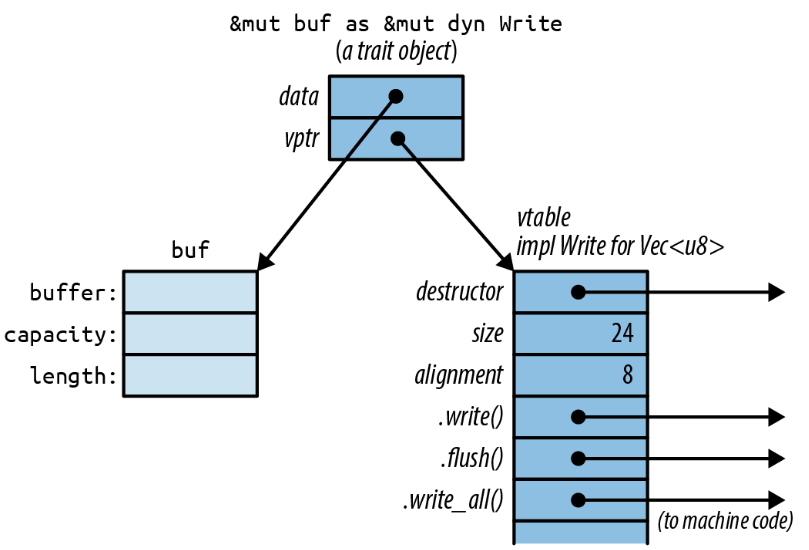
\includegraphics[width=0.9\textwidth]{../img/f11-1.png}
    \caption{内存中的trait对象}
    \label{f11-1}
\end{figure}

C++也有这种运行时的类型信息。它被称为\emph{虚表}或者\emph{vtable}。在Rust中和在C++中一样,vtable只会在编译期生成一次,然后被所有相同类型的对象共享。\hyperref[f11-1]{图11-1}中较深颜色的阴影显示的内容,包括vtable,都是Rust的私有实现。这些字段和数据结构你不能直接访问。当你调用trait对象的方法时语言本身会自动使用vtable来决定要调用哪个实现。

熟练的C++程序员可能会注意到Rust和C++采取的内存策略有些不同。在C++中,虚表指针或者称为\emph{vptr}被存储为结构体的一部分,而Rust使用胖指针来代替。结构体本身不包含任何自身字段之外的东西。这样,一个结构体可以实现一大堆trait而不需要包含一大堆vptr。即使像\texttt{i32}这样的大小还不足以容纳一个vptr的类型,也可以实现trait。

当需要时Rust会自动把普通引用转换为trait对象。这就是为什么我们能在这个例子中直接把\texttt{\&mut local_file}传递给\texttt{say\_hello}:
\begin{minted}{Rust}
    let mut local_file = File::create("hello.txt")?;
    say_hello(&mut local_file)?;
\end{minted}

\texttt{\&mut local\_file}的类型是\texttt{\&mut File},而\texttt{say\_hello}的参数类型是\texttt{\&mut dyn Write}。因为\texttt{File}是一种writer,所以Rust允许这种普通引用到trait对象的转换。

同样的,Rust也乐于把\texttt{Box<File>}转换成\texttt{Box<dyn Write>},它拥有一个在堆上的writer:
\begin{minted}{Rust}
    let w: Box<dyn Write> = Box::new(local_file);
\end{minted}

\texttt{Box<dyn Write>}类似于\texttt{\&mut dyn Write},是一个胖指针:它包含writer自身的地址和vtable的地址。其他指针类型例如\texttt{Rc<dyn Write>}也一样。

这种转换是唯一创建trait对象的方法。编译器做的工作其实很简单,当转换发生时,Rust知道被引用值的真正类型(这个例子中是\texttt{File}),因此它只是加上了正确的vtable的地址、把普通指针变成了胖指针。

\subsection{泛型函数和类型参数}


\section{完全限定方法调用}\label{fullymethod}

